\section{Resultat}

De frågeställningar som ställdes i början av dokumentet var:
\begin{enumerate}
\item Går det att implementera en kvadratisk optimeringslösare i programspråket C?
\item Kan kandidatgruppen implementera ett system som löser kvadratiska optimeringsproblem snabbare än Gurobi?
\item Kan projektet utföras utan någon speciell utvecklingsmetodik? 
\end{enumerate}

Svaren på dessa frågor besvaras i listan nedan:
\begin{enumerate}
\item Ja, det går att implementera en kvadratisk optimeringslösare i programspråket C med den tid som hade getts. Den kvadratiska optimeringslösaren som skrevs i programspråket C var Active set metoden. I figur \ref{fig:arkitektur} visas en överblick hur hela systemet såg ut. Där solution.c skapar en struct innehållande de matriser som problemet består av och sedan löser solvern detta problem.

\begin{figure}[h]
\centerline{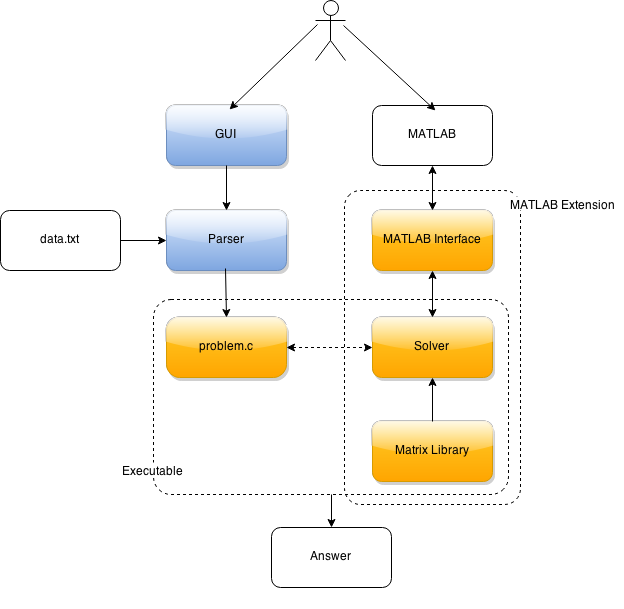
\includegraphics[scale=0.5]{grafik/arkitektur}}
\caption{Grafisk representation av lösningen}
\label{fig:arkitektur}
\end{figure}

\item Nej, ett system som kan lösa kvadratiska optimeringsproblem snabbare än Gurobi kan inte utvecklas med den tid som har funnits till hands. Kandidatgruppens sju medlemmar hade 270 timmar var att fördela projektet på, varav många timmar lades ner på dokumentation och diverse seminarier. Utan dokumentation och seminarier skulle optimeringsalgoritmen kunnat blivit bättre.

\item Ja, projektet kan utföras utan någon konkret utvecklingsmetodik. Däremot så kan man arbeta efter en viss utvecklingsmetodik utan att veta om det, dvs en skräddarsydd utvecklingsmetodik. Kandidatgruppen i detta fall gick in i iterationerna utan en utvecklingsmetodik, men under arbetsgången skapades en sorts utvecklingsmetodik som hjälpte till att utveckla optimeringsalgoritmen.
\end{enumerate}
	
	
\subsection{Kandidatgruppens gemensamma erfarenheter}
En lärdom kandidatgruppen tagit under projektets gång är vikten av att hålla regelbundna möten med kunden i början av projektet för att klargöra vad som verkligen ska göras. Många frågor uppkommer och utan en tydlig kravspecifikation blir det svårt att planera projektet. Den första kravspecifikationen som togs fram var bristfällig då gruppmedlemmarna saknade praktisk erfarenhet av dels kvadratiska optimeringsproblem och dels metodiker för programvaruutveckling. Om fler kundmöten hade planerats hade åtminstone det förstnämnda blivit ett mindre problem. Istället blev det mycket osäkerheter kring uppgiften i början av projektet vilket ledde till att kandidatgruppen förlorade tid. Till exempel försöktes lösningsalgoritmen implementeras utan tillräcklig kunskap vilket gjorde att den behövde revideras flera gånger.
\newline
\newline
Kandidatgruppen har haft goda erfarenheter med att använda molntjänster som GitHub och Google Drive för hantering av kod och dokumentation, så länge kandidatgruppen gör upp vilka som skriver vad för att undvika konflikter i versionshanteringen. När konflikter har uppstått har de tacklats med utbildning av kandidatgruppens samtliga medlemmar, vilket har lett till mer kunskapsspridning.
\newline
\newline
Till yttermera visso har kandidatgruppen fått en djupare förståelse för programspråket C. Då ett krav på programvaran är att den ska gå att kompilera och exekvera på ett flertal plattformar, har kandidatgruppen fått en insikt om vad ''implementation defined'' verkligen betyder. Det har hänt flera gånger att programmet går att exekvera på en plattform men får segmenteringsfel på en annan. Detta beror ofta på att olika operativsystem och kompilatorer hanterar minnesallokering på olika sätt.
\newline
\newline
Utöver detta har kandidatgruppen insett vikten av testning och kontinuerlig integration. Tack vare att ett synnerligen välfungerande byggsystem implementerades tidigt i projektets gång har mycket tid sparats in som antagligen skulle lagts på kompilering och felsökande. Kandidatgruppens byggserver kör automatiskt tester direkt när kod har skickats till den centrala versionshanteringsservern och varnar syndaren via elektronisk post om något test eller kompilering skulle misslyckas. Detta har gjort att fel har upptäckts tidigt och åtgärdats snabbt.

\subsection{Översikt över de individuella utredningarna}
I de individuella utredningarna har kandidatgruppen rapporter som behandlar: 
\begin{itemize}
	\item En undersökning av olika byggsystem.
	\item Hur man är en bra team ledare och vad best practices är.
	\item Optimering av matrisbibliotek. 
	\item {\LaTeX} i ett programmeringsprojekt.
	\item Testning av mjukvara. 
	\item Hur man tar fram en bra arkitektur. 
	\item Kvalitetssäkring i ett projekt.  
\end{itemize}
Dessa individuella delar bygger på antingen författarens roll eller ett område författaren ägnat mycket av sin tid åt under projektets gång. I de fall där den individuella delen baseras på en roll har författaren valt att rikta in sig på en specifik del av rollen som är kopplad till projektet. De resterande områden som skrivits om har inte enbart varit ett område där författaren lagt mycket utav sin tid utan det är även områden som projektet har gynnats mycket av.
